
%%!TEX root = ./heapvis.tex

\section{Future Work}
\label{future}

We have demonstrated Heapviz's performance on large programs; however, our
summarization algorithm cannot greatly compress the size of graphs for programs
containing a large number of nodes that have unique predecessor sets.  With
highly-connected graphs, such as the SPEC JBB 2000 benchmark
(Figure~\ref{fig:jbb}), it is difficult to see the results of a query, even
with highlighting of the relevant nodes.  Our current summarization algorithm
applies the same set of rules for merging nodes to all heap graphs, regardless
of complexity.  We plan to experiment with adjustable levels of detail,
in which the summarization algorithm applies increasingly-powerful abstraction
rules to a graph until it reaches a certain threshold of complexity, 
measured in number of nodes and edges.  For example, Heapviz currently
preserves sharing information among nodes, but for complex graphs
like SPEC JBB 2000 it could discard sharing information to produce a more
manageable visualization.

\looseness -1
On a similar note, our visualization currently allows users to collapse and
expand nodes based on the dominator tree.  Another possibility would be
to expand and collapse the concrete nodes that a particular summary 
node represents.
This approach would require care to ensure that the graph does not become
too complex when a summary node is expanded.

Heapviz currently supports searching for nodes by type, but a full-fledged
query language would allow users to search for objects that meet specific
criteria.  We envision a query language based on first-order logic, similar
to the heap assertion language proposed by Reichenbach et 
al.~\cite{reichenbach10deal}.  Such a
language would allow queries such as ``Which objects of type \texttt{String} 
have $\texttt{length} \geq 5$?'' and ``Which objects are reachable from object 
\texttt{a}?''  Similarly, we could support a path query language to highlight
paths through the heap that match certain criteria.

Finally, because our long-term goal with Heapviz is to produce a tool that 
will be useful to developers, we intend to release Heapviz to the developer community.
In order to reach this goal, we plan to conduct formal user studies to determine
what improvements Heapviz requires before even an early version can be released.

\begin{figure}[t]
  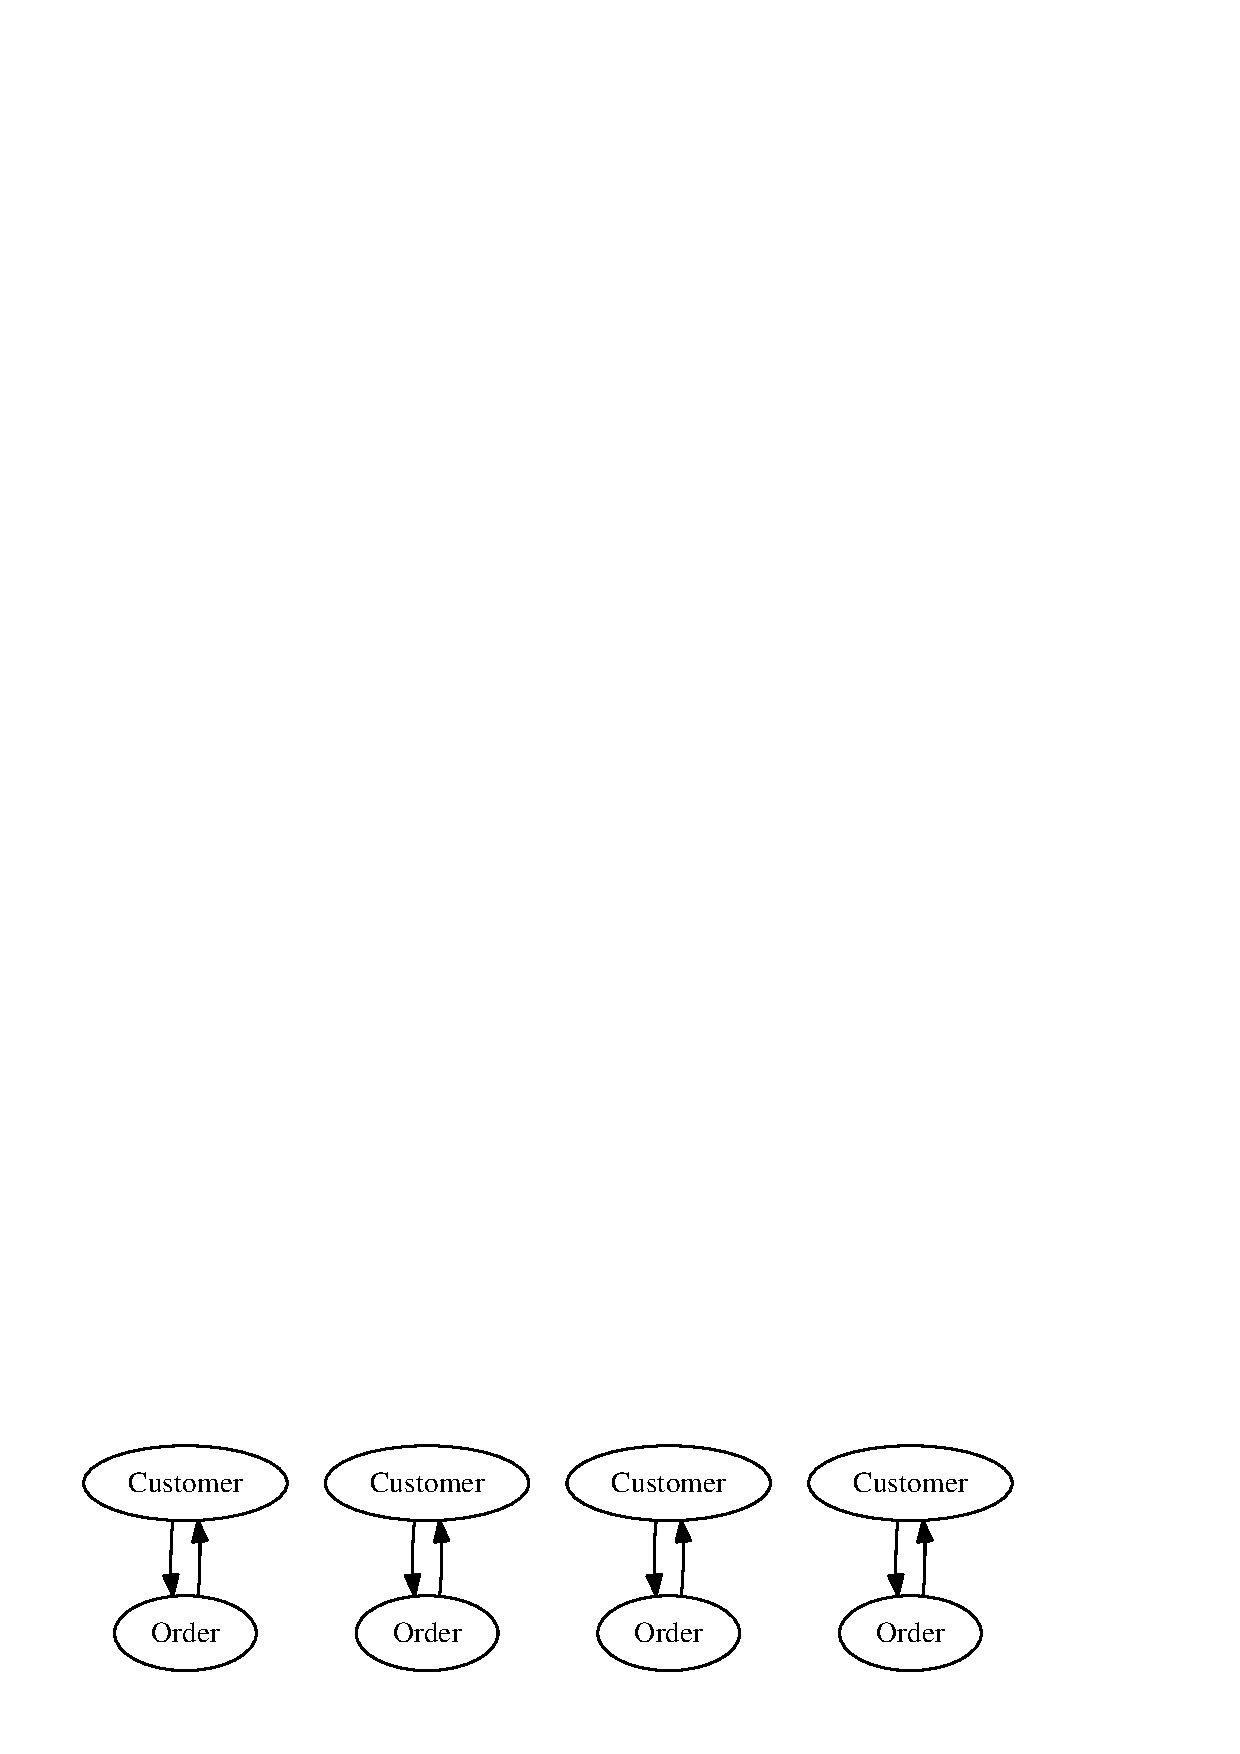
\includegraphics[width=\columnwidth]{figs/failure}
  \caption{An example of the one-to-one mapping between ``leaf'' elements
that we observed in SPEC JBB 2000.  No matter what other objects point to
these objects, they will not be summarized because the one-to-one structure
guarantees that each has a unique predecessor set.}
  \label{fig:failure}
\end{figure}

%\todo{AG: If you're looking to add examples (which you may not), you might want
%to compare the same heap in two location in the program. Could that help you
%interpret some of the actions in the program? Or have a visual indication of
%how the program grows (either by size of summarized graph, or amount of
%elements merged, etc.)?  Goes with the question of whether you can get multiple
%heap dumps in a single program.} 

\section{Conclusions}
\label{conclusions}

We have presented a tool for helping programmers analyze, visualize,
and navigate heap snapshots from running Java programs.  Heapviz enables users
to navigate large, pointer-based data structures at a whole-program scale.  We
have introduced a heap analyzer, which parses a heap snapshot, builds a graph
representation, and applies algorithms to create a summarized heap abstraction.
We have demonstrated how to navigate this abstraction with a heap visualizer
which supports several interaction styles, including detailed field view,
expanding and collapsing of nodes, edge visibility toggles, and search.

Heapviz builds on a body of prior work on tools for debugging, static analysis,
and data structure visualization.  Our system makes several key contributions.
Unlike traditional debuggers, we provide both an overview and detail; Heapviz
provides the global view of the actual heap contents, as well as the ability to
examine detail on demand with the field view.  
%In addition, by visualizing the actual heap snapshot, we overcome the
%limitations faced by static analysis tools: we sidestep the problems related
%to dynamic software architectures, and we avoid the inherent limitations of
%heap approximation. 
This variable level of detail supports programmer productivity in many common
usage scenarios, including finding bugs and memory leaks, identifying data
structures that could be improved, and understanding the overall system
architecture.  We hope that further exploration of domain-specific usage
scenarios will spark the development of new analysis and visualization
techniques.
